\documentclass[a4,useAMS,usenatbib,usegraphicx,12pt]{article}
%External Packages and personalized macros
%=========================================================================
%		EXTERNAL PACKAGES
%=========================================================================
\usepackage[round]{natbib}
\usepackage[margin=3cm]{geometry}
\usepackage{hyperref}
\usepackage{times}
\usepackage{amsmath} 
\usepackage{amssymb}
\usepackage{graphicx}
\usepackage{array, xcolor, bibentry}

\definecolor{lightgray}{gray}{0.8}
\newcolumntype{L}{>{\raggedleft}p{0.14\textwidth}}
\newcolumntype{R}{p{0.8\textwidth}}
\newcommand\VRule{\color{lightgray}\vrule width 0.5pt}

\usepackage{booktabs}% http://ctan.org/pkg/booktabs
\newcommand{\tabitem}{~~\llap{\textbullet}~~}

%=========================================================================
%		INTERNAL MACROS
%=========================================================================
% To highlight comments 
\definecolor{red}{rgb}{1,0.0,0.0}
\newcommand{\red}{\color{red}}
\definecolor{darkgreen}{rgb}{0.0,0.5,0.0}
\newcommand{\SRK}[1]{\textcolor{darkgreen}{\bf SRK: \textit{#1}}}
\newcommand{\SRKED}[1]{\textcolor{darkgreen}{\bf #1}}

\newcommand{\LCDM}{$\Lambda$CDM~}
\newcommand{\beq}{\begin{eqnarray}}  
\newcommand{\eeq}{\end{eqnarray}}  
\newcommand{\zz}{$z\sim 3$} 
\newcommand{\apj}{ApJ}  
\newcommand{\apjs}{ApJS}  
\newcommand{\apjl}{ApJL}  
\newcommand{\aj}{AJ}  
\newcommand{\mnras}{MNRAS}  
\newcommand{\mnrassub}{MNRAS accepted}  
\newcommand{\aap}{A\&A}  
\newcommand{\aaps}{A\&AS}  
\newcommand{\araa}{ARA\&A}  
\newcommand{\nat}{Nature}  
\newcommand{\physrep}{PhR}
\newcommand{\pasp}{PASP}    
\newcommand{\pasj}{PASJ}    
\newcommand{\avg}[1]{\langle{#1}\rangle}  
\newcommand{\ly}{{\ifmmode{{\rm Ly}\alpha}\else{Ly$\alpha$}\fi}}
\newcommand{\hMpc}{{\ifmmode{h^{-1}{\rm Mpc}}\else{$h^{-1}$Mpc }\fi}}  
\newcommand{\hGpc}{{\ifmmode{h^{-1}{\rm Gpc}}\else{$h^{-1}$Gpc }\fi}}  
\newcommand{\hmpc}{{\ifmmode{h^{-1}{\rm Mpc}}\else{$h^{-1}$Mpc }\fi}}  
\newcommand{\hkpc}{{\ifmmode{h^{-1}{\rm kpc}}\else{$h^{-1}$kpc }\fi}}  
\newcommand{\hMsun}{{\ifmmode{h^{-1}{\rm {M_{\odot}}}}\else{$h^{-1}{\rm{M_{\odot}}}$}\fi}}  
\newcommand{\hmsun}{{\ifmmode{h^{-1}{\rm {M_{\odot}}}}\else{$h^{-1}{\rm{M_{\odot}}}$}\fi}}  
\newcommand{\Msun}{{\ifmmode{{\rm {M_{\odot}}}}\else{${\rm{M_{\odot}}}$}\fi}}  
\newcommand{\msun}{{\ifmmode{{\rm {M_{\odot}}}}\else{${\rm{M_{\odot}}}$}\fi}}  
\newcommand{\lya}{{Lyman$\alpha$~}}
\newcommand{\clara}{{\texttt{CLARA}}~}
\newcommand{\rand}{{\ifmmode{{\mathcal{R}}}\else{${\mathcal{R}}$ }\fi}}  


%MY COMMANDS #############################################################
\newcommand{\sub}[1]{\mbox{\scriptsize{#1}}}
\newcommand{\dtot}[2]{ \frac{ d #1 }{d #2} }
\newcommand{\dpar}[2]{ \frac{ \partial #1 }{\partial #2} }
\newcommand{\pr}[1]{ \left( #1 \right) }
\newcommand{\corc}[1]{ \left[ #1 \right] }
\newcommand{\lla}[1]{ \left\{ #1 \right\} }
\newcommand{\bds}[1]{\boldsymbol{ #1 }}
\newcommand{\oiint}{\displaystyle\bigcirc\!\!\!\!\!\!\!\!\int\!\!\!\!\!\int}
\newcommand{\mathsize}[2]{\mbox{\fontsize{#1}{#1}\selectfont $#2$}}
\newcommand{\eq}[2]{\begin{equation} \label{eq:#1} #2 \end{equation}}
\newcommand{\lth}{$\lambda_{th}$ }
%#########################################################################

\setlength\parindent{0pt}

\title{Things to discuss}
\author{}
\date{}
  
\begin{document}
\maketitle

\section{Bondi Accretion}
Is Bondi accretion physically consistent with the disk model I am using for spin evolution?
Is there some possible way to implement other accretion model?


\section{Mass interval in spin parameter evolution}
Checking dependence on mass per accretion episode in equation of spin evolution. The solution
given by (Bardeen, 1970) is exact as any interval gives the same solution. However, this cannot
be randomly chosen in the code as there is a probability of spin-flip in both, the chaotic and
prolonged mode.

%.........................................................................
\begin{figure}[htbp]
\centering
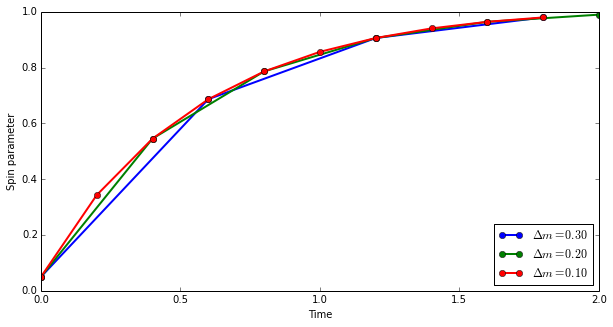
\includegraphics[width=0.7\textwidth]{./figures/SpinEvolution.png}
\end{figure}
%.........................................................................

%.........................................................................
\begin{figure}[htbp]
\centering
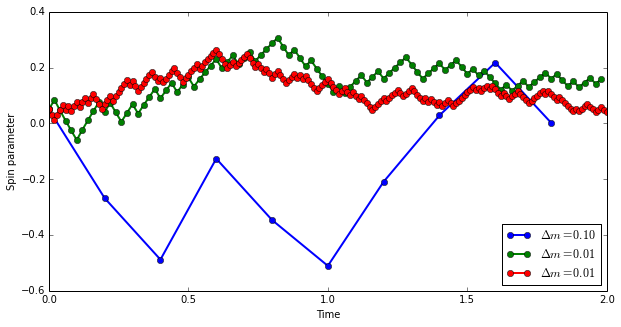
\includegraphics[width=0.7\textwidth]{./figures/SpinEvolutionFlip.png}
\end{figure}
%.........................................................................

\section{Recoil speed}
The recoil velocity after a merger is already working, however there is some issues regarding the
way the two black holes approach to each other. Using the repositioning scheme, sometimes both
BHs are forced to be in the same position at the same time, which makes the code crash. Using the 
drag-force as an approximation of dynamical friction is much better, however as it depends linearly
on the speed of the BH, the kick is quickly compensated. This would be different with the Chandrasekhar
formula, as the faster the BH goes, the fewer stars with a higher speed to slow it down.

%.........................................................................
\begin{figure}[htbp]
\centering
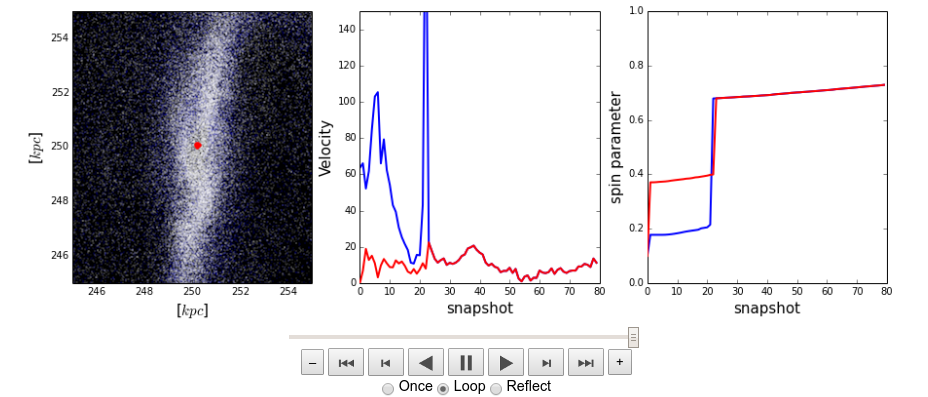
\includegraphics[width=1.\textwidth]{./figures/VideoRecoil.png}
\end{figure}
%.........................................................................

%.........................................................................
\begin{figure}[htbp]
\centering
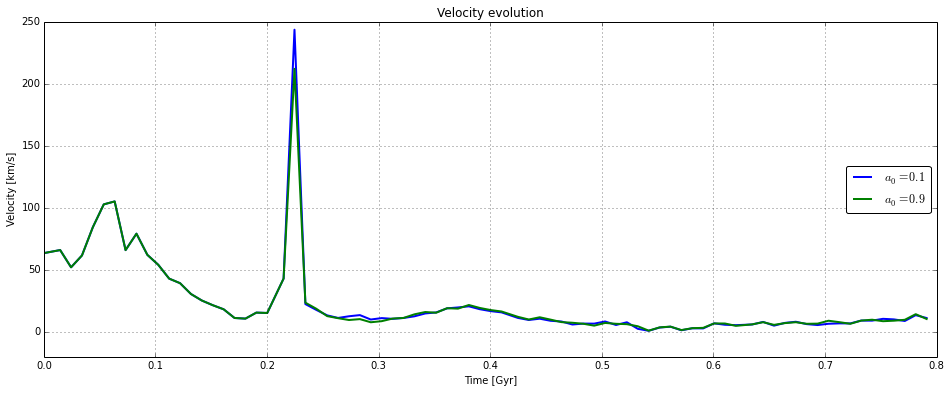
\includegraphics[width=.9\textwidth]{./figures/RecoilSpins.png}
\end{figure}
%.........................................................................

\section{BH mass relation}

I have run four different simulations. The control one with the fiducial model which serves as a control
run. Second, the same fiducial model, but freeing the BHs from the potential centre. The BHmass-Stellar mass
is not reproduced at all as the BHs wander around low density regions, thereby decreasing their accretion 
rates. The third run is the same fiducial model, but introducing spin evolution. The results are basically 
the same as the spin module (without recoils) doesn't have any effect on the physics. Finally, the last run
implements the full spin model, including recoils. However, in order to avoid numerical crashes, the drag-force
dynamical friction is implemented. The BH mass relation is reproduced, but it seems to be more spread out. 
The resolution of the simulation is low though.

%.........................................................................
\begin{figure}[htbp]
\centering
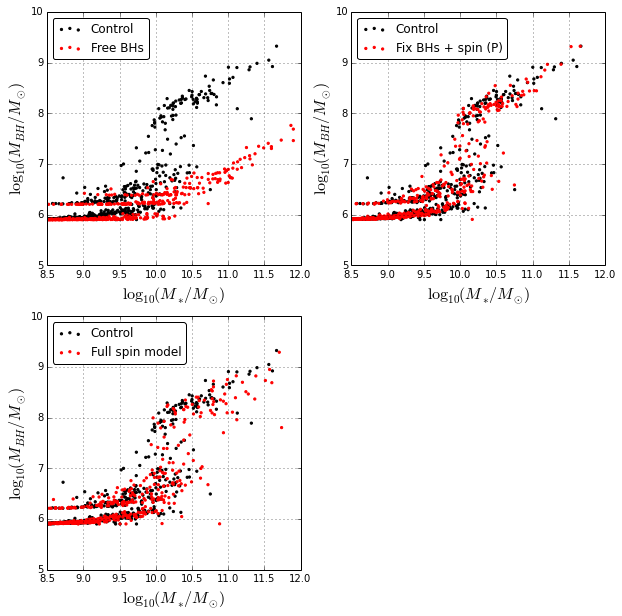
\includegraphics[width=.8\textwidth]{./figures/BHmassRelation.png}
\end{figure}
%.........................................................................


\section{Transition between chaotic and prolonged modes}

Right now I implemented in the code a switch of spin model using the same mass-dependent criterion for the 
quasar or radio mode. However, there seem to be a issue with this. The transition to the radio mode (prolonged
spin mode) from the quasar mode (chaotic spin mode) seems to happen a bit late, where the mass accretion rate
is too low that the spin is basically not evolving during the prolonged mode.


%.........................................................................
\begin{figure}[htbp]
\centering
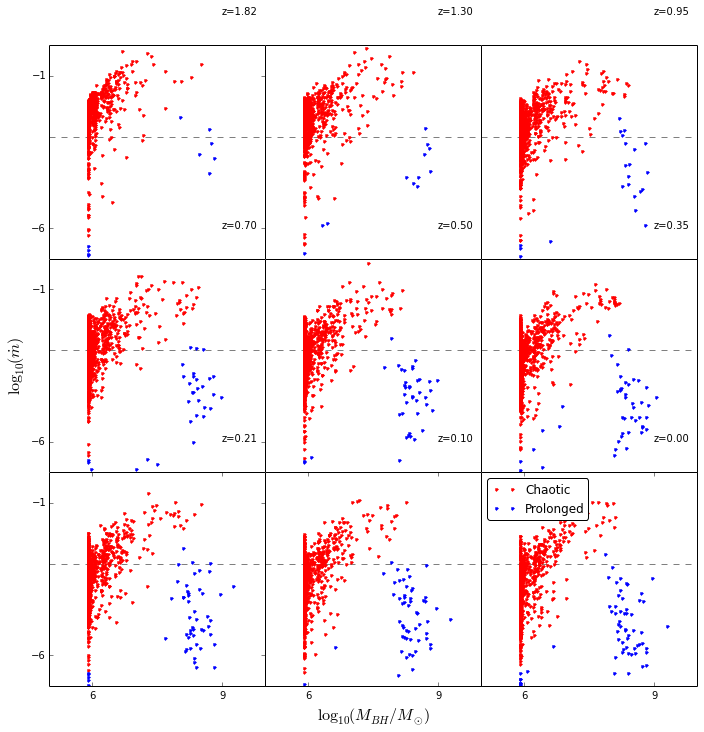
\includegraphics[width=0.8\textwidth]{./figures/MassAccretion.png}
\end{figure}
%.........................................................................

The high spin values reached in the chaotic mode are a result of a bug in the code, where I was using a value 
for the spin of the disk computed with the formula of the prolonged mode, yielding to high values and then
the randomization of the direction of angular momentum was lost, pointing always pointing in the direction of 
the BH's spin. I am running a new simulation where this is corrected. Presumably only low to middle spin values
will be observed. The coalescence of black holes is another mechanism to raise the spin value.

\newpage

%.........................................................................
\begin{figure}[htbp]
\centering
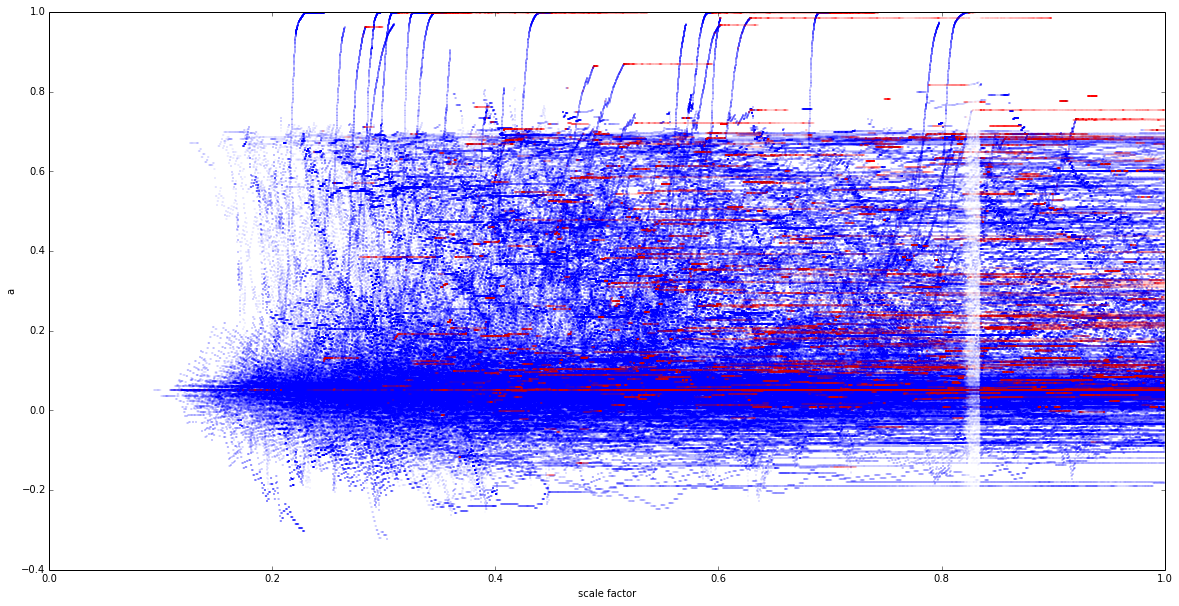
\includegraphics[width=1.0\textwidth]{./figures/SpinEvolutionCosmo.png}
\end{figure}
%.........................................................................


It is perhaps a better idea to apply a new criterion where the mass per episode in both modes are compared. So, 
whatever value is the smallest, the respective mode will be implemented. This has physical sense as the amount
of mass accreted from self-gravitating disk should be smaller than whole mass inside the warped region. The 
question remaining should be whether to apply this only to the spin, or also extending it to the definition of
the quasar/radio mode transition.


%.........................................................................
\begin{figure}[htbp]
\centering
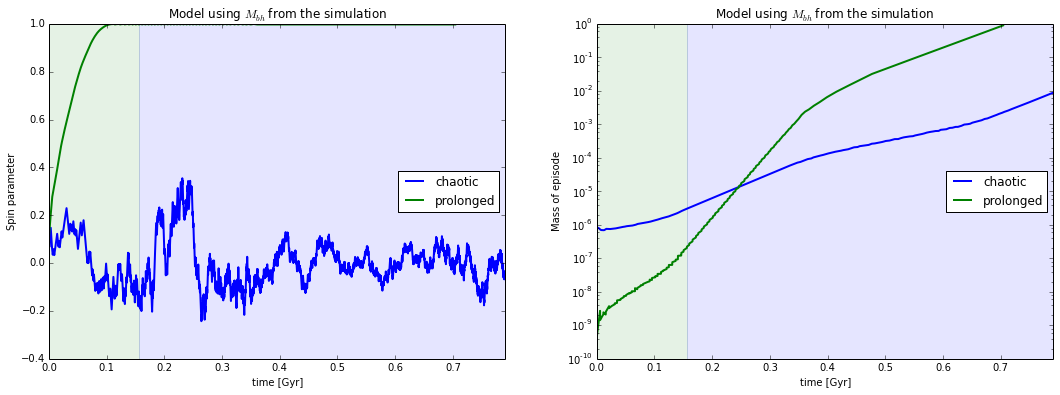
\includegraphics[width=1.0\textwidth]{./figures/TransitionMode.png}
\end{figure}
%.........................................................................


\section{Spin alignment}

I also was trying to study spin alignment as I am able to model direction evolution. At the moment it makes no
much sense as the prolonged mode, where the BH's tend to align to the angular momentum of the neighbouring gas
cells, is not properly working for all the BHs. However, it is interesting to verify that there is a tendency
toward alignment.

%.........................................................................
\begin{figure}[htbp]
\centering
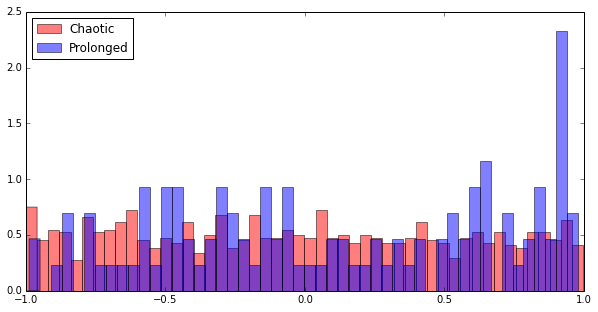
\includegraphics[width=0.7\textwidth]{./figures/Alignment.png}
\end{figure}
%.........................................................................

%.........................................................................
\begin{figure}[htbp]
\centering
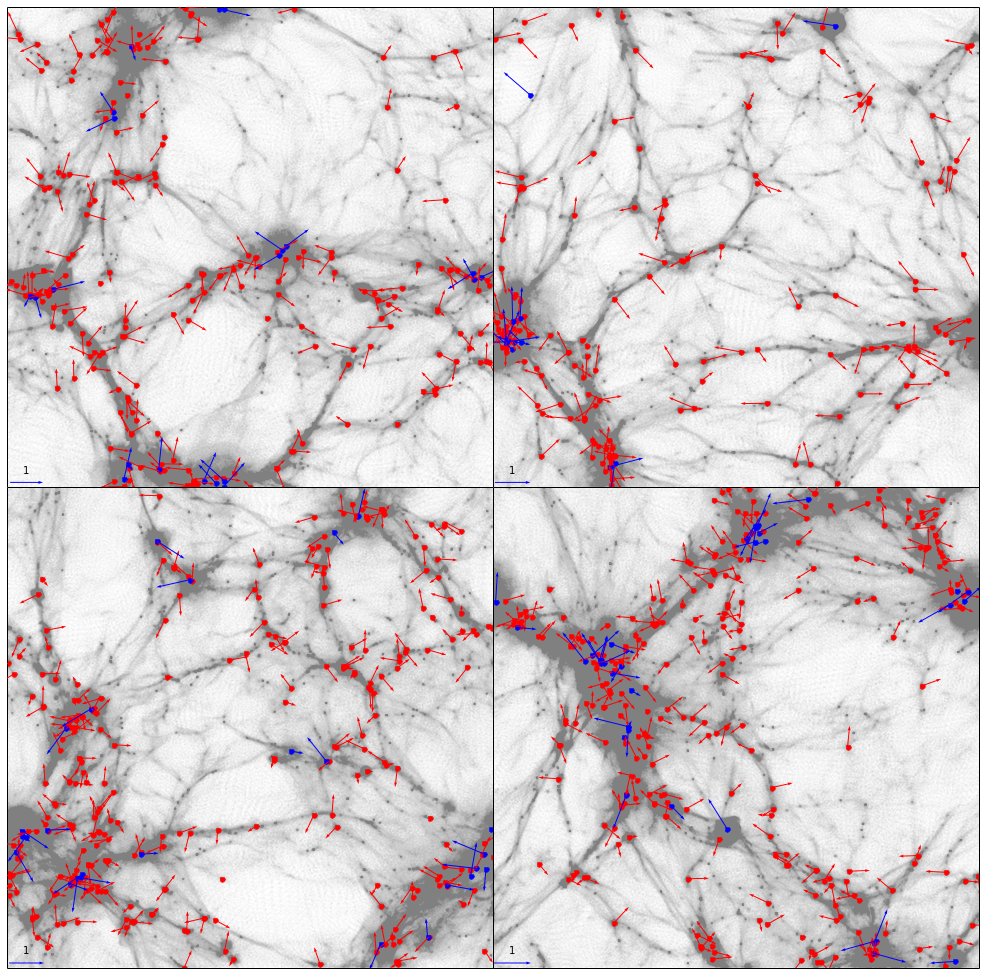
\includegraphics[width=0.9\textwidth]{./figures/Alignment_Spatial.png}
\end{figure}
%.........................................................................

\section{Future work}

\begin{itemize}
 \item Further tests of the model.
 \item Original idea. Study dynamical friction and recoil velocities. This would require to focus on a more 
 realistic dynamical friction treatment.
 \item Spin model itself. Study the spin evolution and the transition between modes. Maybe we can explore a
 new criterion based on the mass per episode. 
 \item As an extension of the previous item, we can study spin-depended accretion efficiencies. This may have
 effects on the BH feedback and more interestingly, on the growth of seeds.
 \item An idea I was discussing with Rainer, which is about using the spin model along with his module of jet emissions.
 For example the jet can be applied in the direction of the spin, and it can also be another mechanism of spin evolution
 as the jet power comes from rotational energy of the BH.
 \item Considering this, it might be interesting to study large-scale alignment of spin (jets) with galaxies and their 
 environment. To this purpose, we can use Jaime's code for calculating the Tweb/Vweb of cosmological simulations.
\end{itemize}



\end{document}
